\section{Analysis}
\label{sec:analysis}

% Your report can include qualitative evaluations. You should try to understand your system (e.g. how it works, when it succeeds and when it fails) by inspecting key characteristics or outputs of your model.
% Types of qualitative evaluation include: commenting on selected examples, error analysis, measuring the performance metric for certain subsets of the data, ablation studies, comparing the behaviors of two systems beyond just the performance metric, and visualizing attention distributions or other activation heatmaps.

% Plan
% - Data centric approach: We hypothesised that fine-tuning model would narrow its focus of knowledge on the scientific MCQA task. But we never observe menaingful performance increases. However, fine-tuning did work as we see, for example, that phi-3 Base attains 90% on ARC train split suggesting it has previously been trained on this dataset. We think that Microsoft's base model has already been trained on all this data, and that they have already done a lot of fine-tuning which we do not manage to meaningfully improve upon.
% - Performance per subject: reduce size
% - Answer distribution: a bit more analysis, what is the distribution of answers in ARC train?

% We hypothesise that it is challenging
% to improve upon our baseline model, as it is already well-suited for MCQA tasks,
% possibly even fine-tuned on the same datasets. In fact, checking the benchmark
% performance on the training splits of the . This suggests, that the model has
% already been fine-tuned on the collection of fine-tuning datasets considered.
% Interestingly though, a "re-finetune" does not seem to lead to the model
% ``focusing'' on the knowledge pertinent to fine-tune datasets and ``forget''
% knowledge irrelevant for the task, which we had hoped for prior to the
% experiments.

\subsection{Lack of Performance Improvement}
\label{subsec:lack-of-performance-improvement}

We hypothesised that fine-tuning the base model Phi-3 on various highly curated MCQA datasets and a custom DPO preference dataset would improve the model's MCQA performance. However, we observe that the fine-tuned models do not outperform the base model. This finding is surprising, as we expected the fine-tuned models to narrow their focus of knowledge on the scientific MCQA task.

We conducted further analysis. The base model Phi-3 attains a mean accuracy of 93.6\% on the ARC training split, strongly suggesting that the base model was already trained on the ARC dataset. By comparison, it attains 69.4\% on the test split. The fine-tuned Phi-3-ARC variant attained an accuracy of 97.6\% on the train split. This improvement over Phi-3 base leads us to believe that fine-tuning did 'narrow' the model's focus. However, this is merely memorisation and does not lead to generalisation, even over the same dataset as Phi-3 curiously does better than Phi-3-ARC on the test split, with Phi-3-ARC attaining an accuracy of 66.3\%.

The fact that the model has likely already been fine-tuned on the datasets we use makes it hard to improve the model performance using the same data. A 're-finetune' does not seem to lead the model to focus on the knowledge pertinent to the fine-tuning datasets which we had hoped for prior to the experiments. It does help a little with pure memorisation, but not with generalisation, even within the same dataset. Microsoft have clearly already struck a good balance over the training datasets to optimise for general reasoning.

\subsection{Qualitative Samples}
\label{subsec:qualitative-samples}

Below is an example of the model's predictions on the ARC dataset using both the Phi-3 and Phi-3-ARC for a sample question.

\begin{lstlisting}[caption={Sample Question}]
Question: Consider the Bayesian network 
given below. How many independent
parameters are needed for this Bayesian 
Network H -> U <- P <- W?
Options:
A. 2
B. 4
C. 8
D. 16
Answer:

--- PHI-3 ---
To determine the number of independent
parameters needed for the Bayesian
network H -> U <- P <- W, we need
to consider the conditional probability
tables (CPTs) for each node given its 
parents. In this network ...

--- PHI-3-ARC ---
The correct answer is C. 8
\end{lstlisting}

We clearly see that the fine-tuned model predicts an answer directly, while the base model provides a detailed explanation. This is expected given the formatting of MCQA text we feed into the model during fine-tuning. Below is another sample for only Phi-3-ARC.

\begin{lstlisting}[caption={Phi-3-ARC sample}]
You: Is Messi the best player ever? 
Phi-3-ARC: The correct answer is A. True
\end{lstlisting}

Interestingly, the model predicts a multiple choice answer to a yes/no question. It has been \emph{over}-fine-tuned and hallucinates a mutliple choice style answer to a question that does not have one. Clearly our fine-tuned models do not generalise well and are overfitted to the training data.

\subsection{Per Subject Analysis}
\label{subsec:performance-per-subject}

To investigate if the model has strengths and weaknesses in different subject areas within STEM, we look at the 19 subjects within the MMLU-Stem benchmark. These include physics, chemistry, biology, and mathematics at different educational levels, such as elementary school, high school, and college. Figure~\ref{fig:mmlu-per-subject} visualises a sample of the mean accuracies per subject. 

% Overall
Overall, we observe that the per-subject performance differs greatly, with models achieving a mean accuracy on High School and College Biology of 83.98\% and 80.79\%, respectively. In contrast, the models perform poorly on high school and college, mathematics and physics, not surpassing 50\% accuracy. This finding could be attributed to two factors: first, the inherent complexity of the subjects and second, the lack of training data for these subjects of the models. Either way, the performance could be improved significantly by collecting more training data for challenging subjects.

% Comparison
The per-subject comparison of the base, fine-tuned and quantised model shows similar trends as the overall benchmark suggests. No clear trends of one model being predictably better in some subjects than others are observed, which is expected since both fine-tuned models were trained on the smae 

\begin{figure}
    \centering
    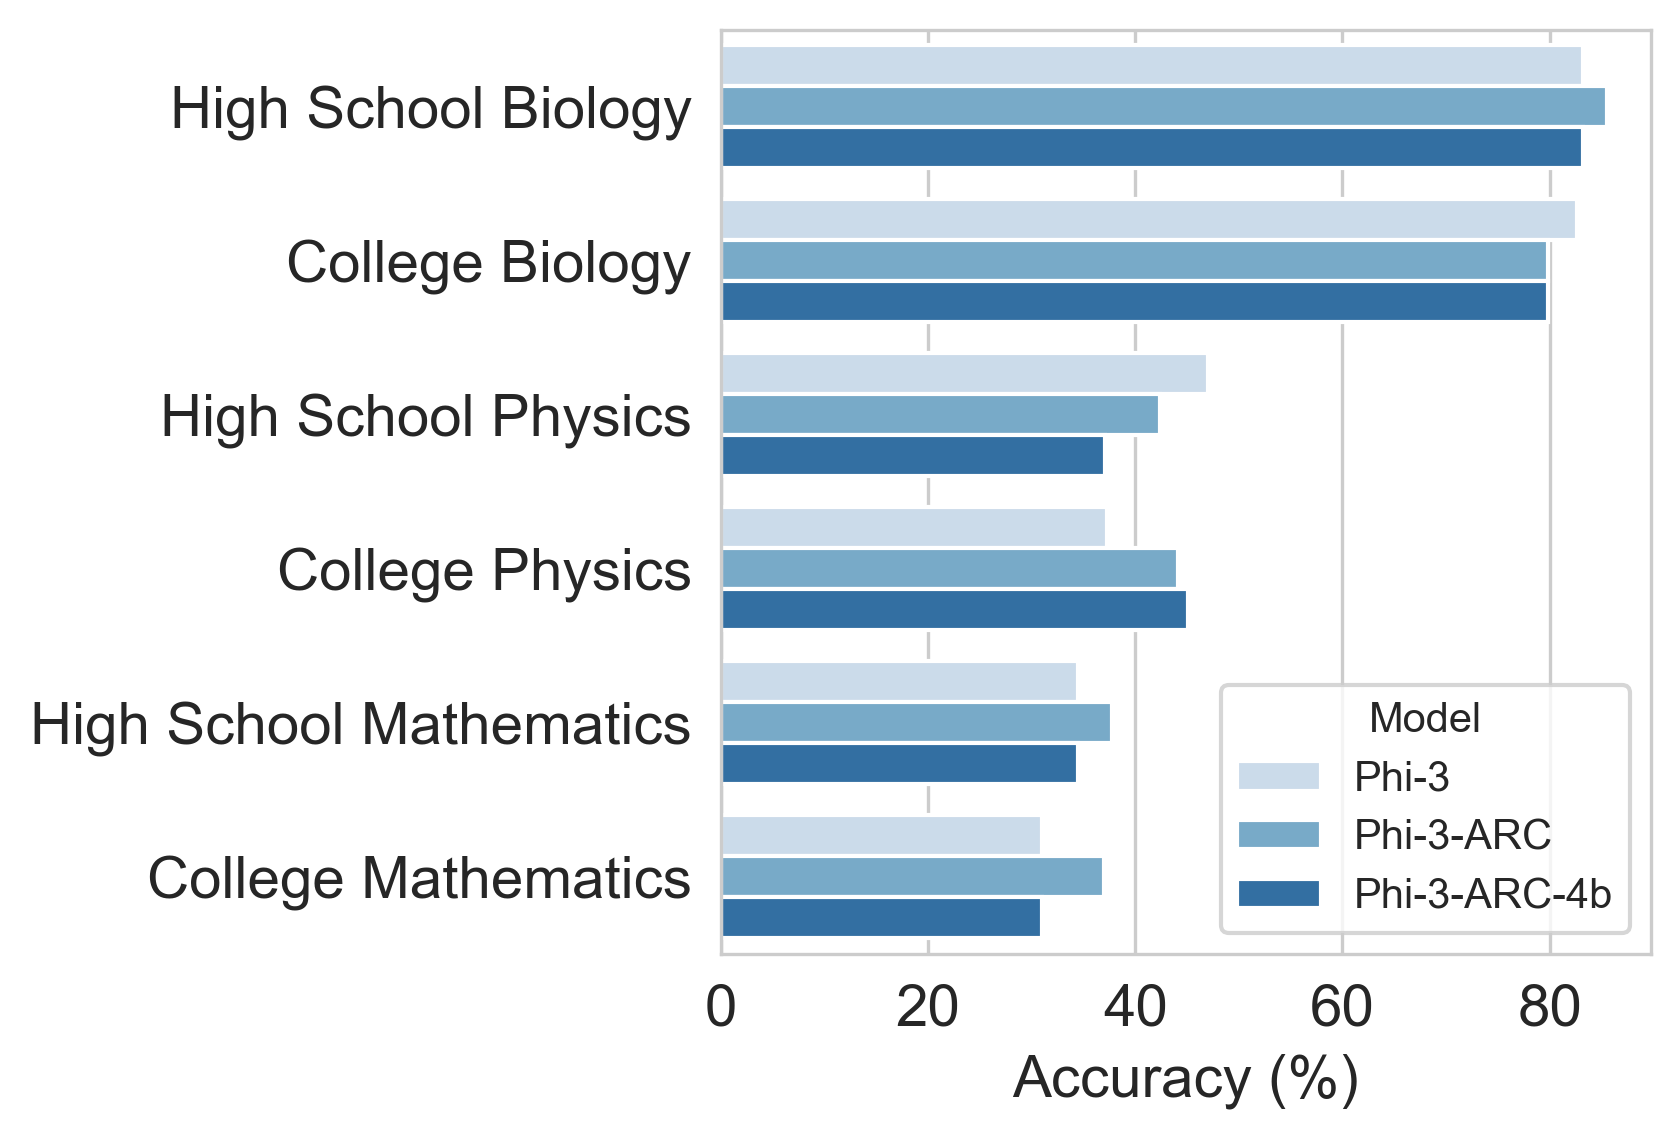
\includegraphics[width=0.45\textwidth]{figures/mmlu-per-subject.png}
    \caption{\textbf{MMLU Per Subject.}
        The mean accuracy of the base model Phi-3, the best performing fine-tuned model Phi-3-ARC, and its 4-bit quantised version Phi-3-ARC-4bit, per subject.
    }
    \label{fig:mmlu-per-subject}
\end{figure}

\subsection{Skewed Answer Distribution}
\label{subsec:answer-distribution}

Next, we investigate the distribution of answers of the three models under
consideration. Figure~\ref{fig:mmlu-answer-distribution} shows the heatmap of
the confusion matrix of correct and predicted answers for the base model Phi-3,
and the difference in confusion matrices between the fine-tuned model Phi-3-ARC
and the base model Phi-3, and the quantised model Phi-3-ARC-4bit and the base
model Phi-3. 

Interestingly, we observe that the base model is biased towards answering B, as
indicated by the high number of false positives in the second column. Roughly
30\% of the model's answers are B, despite the true answer distribution being
close to uniform. Moreover, the fine-tuned model Phi-3-ARC, further increases
this bias, perhaps due to the ARC dataset being slightly biased towards B itself. 
Curisouly, quantising the model to 4 bits flattens the distribution
of answers slightly, decreasing the bias towards B.

\begin{figure}
    \centering
    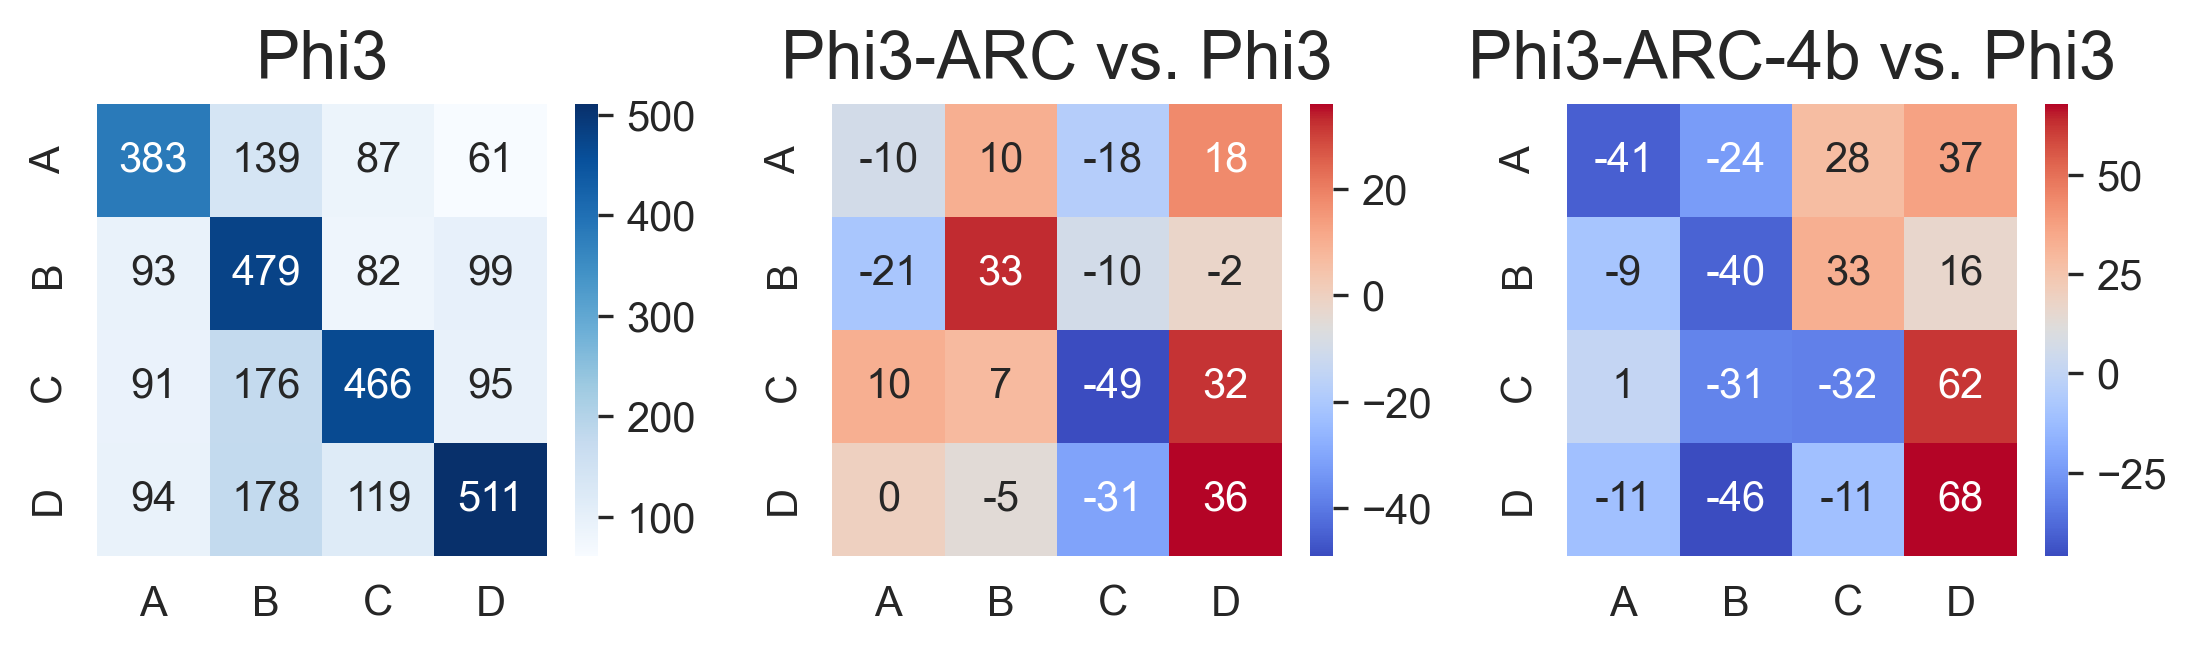
\includegraphics[width=0.45\textwidth]{figures/mmlu-confusion.png}
    \caption{\textbf{
        Confusion Matrics.}
        The confusion matrix of answers given by the baseline model and the difference in accuracy between the fine-tuned model and the baseline model.
    }
    \label{fig:mmlu-answer-distribution}
\end{figure}